% -------------------------------------------------------------------- %
% -------------------------------------------------------------------- %
% -------------------------------------------------------------------- %

\documentclass[twocolumn,10pt]{article} % here we use the article class, rather than elsarticle

% -------------------------------------------------------------------- %
% -------------------------------------------------------------------- %
% -------------------------------------------------------------------- %

\usepackage[square,numbers,sort&compress,comma]{natbib}

\usepackage{amsmath}
\usepackage{amssymb}
\usepackage{xcolor}
\usepackage{caption}
\usepackage{graphicx}
\usepackage{latexsym}
\usepackage{times}
\usepackage{dblfloatfix}
\usepackage{mathabx}

% -------------------------------------------------------------------- %
% -------------------------------------------------------------------- %
% -------------------------------------------------------------------- %

\topmargin - 12pt % might need to be set to 0pt for some installations
\oddsidemargin 32pt
\textheight 610pt
\textwidth 408pt
\columnsep 24pt

% -------------------------------------------------------------------- %
% -------------------------------------------------------------------- %
% -------------------------------------------------------------------- %

\def\thepage{}

\renewenvironment{abstract}%
              {% - begin definition
               \small% - select font
               {\bfseries \abstractname}% - select font
               \par% - end a paragraph (skip \parsep)
               \vspace{10pt}% - add vertical space
              }% - complete definition

\renewcommand\abstractname{Abstract}

\newcommand{\nomenclature}% - name of command
              [1]% - number of arguments
              {% - begin definition
               \bgroup% - begin a local group
               \flushleft% - turn on flushleft option
               \small\bf% - select font
               #1% - insert title text
               \par% - end a paragraph (skip \parsep)
               \egroup% - terminate local group
              }% - complete definition

\renewcommand{\section}% - name of command
              [1]% - number of arguments
              {% - begin definition
               \bgroup% - begin a local group
               \flushleft% - turn on flushleft option
               \small\bf% - select font
               \stepcounter{section}% - increment counter
               \arabic{section}. #1% - insert title text
               \par% - end a paragraph (skip \parsep)
               \egroup% - terminate local group
              }% - complete definition

\renewcommand{\subsection}% - name of command
              [1]% - number of arguments
              {% - begin definition
               \bgroup% - begin a local group
               \flushleft% - turn on flushleft option
               \small\em% - select font
               \stepcounter{subsection}% - increment counter
               \arabic{section}.% - insert title text
               \arabic{subsection}. #1% - insert title text
               \par% - end a paragraph (skip \parsep)
               \egroup% - terminate local group
              }% - complete definition

\renewcommand{\subsubsection}% - name of command
              [1]% - number of arguments
              {% - begin definition
               \bgroup% - begin a local group
               \flushleft% - turn on flushleft option
               \small\em% - select font
               \stepcounter{subsubsection}% - increment counter
               \arabic{section}.% - insert title text
               \arabic{subsection}.% - insert title text
               \arabic{subsubsection}. #1% - insert title text
               \par% - end a paragraph (skip \parsep)
               \egroup% - terminate local group
              }% - complete definition

  \newcommand{\acknowledgement}% - name of command
              [1]% - number of arguments
              {% - begin definition
               \bgroup% - begin a local group
               \flushleft% - turn on flushleft option
               \small\bf% - select font
               #1% - insert title text
               \par% - end a paragraph (skip \parsep)
               \egroup% - terminate local group
              }% - complete definition

  \newcommand{\sectionbib}% - name of command
              [1]% - number of arguments
              {% - begin definition
               \bgroup% - begin a local group
               \flushleft% - turn on flushleft option
               \small\bf% - select font
               #1% - insert title text
               \par% - end a paragraph (skip \parsep)
               \egroup% - terminate local group
              }% - complete definition

\renewcommand\figurename{Fig.}
\renewcommand{\captionsize}{\footnotesize}
\setlength\abovecaptionskip{0pt}
\setlength\belowcaptionskip{0pt}

\renewcommand\bibsection{\sectionbib{\refname}}

\setlength\bibsep{0pt}

\pagenumbering{arabic}

% -------------------------------------------------------------------- %
% -------------------------------------------------------------------- %
% -------------------------------------------------------------------- %

\begin{document}

\title{\LARGE Mitigation of thermoacoustic instability in \\
                     a turbulent combustor via self-coupling}

\author{{\large Ankit Sahay$^{*}$, Abhishek Kushwaha$$, Samadhan A. Pawar$$, \\ P. R. Midhun$$, Jayesh M. Dhadphale$$, R. I. Sujith }\\[10pt]
        {\footnotesize \em Department of Aerospace Engineering, Indian Institute of Technology Madras, Chennai 600036, India }\\[-5pt]}

\date{}

% -------------------------------------------------------------------- %
% -------------------------------------------------------------------- %
% -------------------------------------------------------------------- %

\small
\baselineskip 10pt

% -------------------------------------------------------------------- %
% -------------------------------------------------------------------- %
% -------------------------------------------------------------------- %

\twocolumn[\begin{@twocolumnfalse}
\vspace{50pt}
\maketitle
\vspace{40pt}
\rule{\textwidth}{0.5pt}
\begin{abstract} % 100 to 300 words.
%
In this paper, we report the first observation of complete mitigation of thermoacoustic instability in a bluff-body stabilized turbulent combustor through the method of self-coupling. Self-coupling is achieved by coupling the acoustic field of the combustor to itself through a coupling tube. We characterize the effects of such acoustic self-feedback on the thermoacoustic instability of the system by varying the length and diameter of the coupling tube. We observe that the amplitude and the dominant frequency of the acoustic pressure fluctuations gradually decrease as the length of the coupling tube is increased. A complete suppression of thermoacoustic instability is observed when the coupling tube length is nearly 1.5 times the combustor length. Meanwhile, as we approach the suppression of thermoacoustic instability, the dynamical behavior of acoustic pressure changes from the state of limit cycle oscillations to low amplitude aperiodic oscillations via intermittency. We also study the coupling between the acoustic field and the unsteady flame dynamics for different conditions of self-coupling in the combustor. As the combustor approaches the state of complete suppression, the temporal synchrony between the acoustic pressure and the global heat release rate signals changes from the state of synchronized periodicity to desynchronized aperiodicity through intermittent synchronization. From the spatiotemporal analysis of the combustor flow field, we find complete disruption of the coherent spatial structures of acoustic energy production observed during the state of thermoacoustic instability when the combustor is self-coupled with a tube of optimized size. Thus, we anticipate self-coupling to be a viable option to mitigate high amplitude thermoacoustic oscillations in turbulent combustion systems present in gas turbines and rocket engines.
%
\end{abstract}
\vspace{10pt}
\parbox{1.0\textwidth}{\footnotesize {\em Keywords:} Thermoacoustic instability; Suppression; Self-coupling; Delayed acoustic feedback; Synchronization}
\rule{\textwidth}{0.5pt}
\vspace{10pt}
% {\footnotesize $^*$ Corresponding Author. Email: ankitsahay02@gmail.com}\\
\end{@twocolumnfalse} ]

% -------------------------------------------------------------------- %
% -------------------------------------------------------------------- %
% -------------------------------------------------------------------- %

\clearpage

\section{Introduction} \addvspace{10pt}

Thermoacoustic instabilities have proven to be a major deterrence to the development of low-emission gas turbine engines used for power generation and propulsion applications \cite{lieuwen2005combustion}. Such instabilities lead to ruinously large amplitude pressure oscillations established when positive feedback is developed between the acoustic field and the heat release rate fluctuations in the reaction field of the combustor \cite{sujith2021thermoacoustic}. The presence of these instabilities results in serious performance losses, structural damages, and reduced operational range \cite{culick2006unsteady}. As a result, it is necessary to find ways to mitigate thermoacoustic instabilities in the course of developing new dynamically stable combustion systems.

Traditionally, different mechanisms of closed-loop and open-loop active controls have been developed for  suppressing thermoacoustic instability \cite{dowling2005feedback}. However, these methods suffer from several limitations, such as the use of complex electro-mechanical components, lack of reliability of sensors while operating in the harsh environment of practical combustors, and high maintenance and replacement costs. Another way to mitigate thermoacoustic instabilities is to use passive damping devices such as Helmholtz resonators, perforated liners, quarter and half-wave resonators \cite{zhao2015review}, and Herschel-Quincke tubes \cite{park2008thermo, rajaram2012attenuation}. Despite their limited range of operation, engine manufactures have to rely on these devices to suppress thermoacoustic instability in practical combustors \cite{lieuwen2005combustion}.% \cite{bellucci2004use}. 

Recently, a method from synchronization theory, called mutual coupling of oscillators, has been adopted to suppress thermoacoustic instabilities in two or more systems \cite{sujith2021thermoacoustic}. At appropriate coupling parameter values, coupled systems approach the same  state of oscillation quenching, known as amplitude death \cite{zou2021quenching}. Through experimental and numerical analysis, amplitude death and partial amplitude death have been discovered in coupled laminar thermoacoustic systems \cite{thomas2018effect1, dange2019oscillation, hyodo2020suppression, srikanth2021dynamical}. In addition, a few studies have investigated the dynamics of mutually coupled turbulent combustors \cite{thomas2018effect, jegal2019mutual, moon2020mutual, guan2021low}, and have also reported the presence of amplitude death in them \cite{jegal2019mutual}. Here, the mutual coupling between the systems is achieved by using one (or more than one) tube of a fixed length and diameter. An increase in the length of the coupling tube correspondingly increases the delay time in the coupling of the acoustic fields in the systems \cite{dange2019oscillation, sahay2021dynamics}.

In contrast to the aforementioned studies, in this paper, we present the first application of a novel variant of mutual coupling, known as self-coupling \cite{just1997mechanism}, to mitigate thermoacoustic instabilities in a single turbulent combustion system. Here, the self-coupling is achieved by feeding back the acoustic field of the combustor to itself through a coupling tube. This method has recently been used by a few researchers to suppress limit cycle oscillations in the acoustic field of different systems, such as electro-acoustic system \cite{biwa2016suppression}, acoustic pipeline \cite{lato2019passive}, and horizontal Rijke tube \cite{srikanth2021selfcoupling}, that do not involve turbulent flow. These studies have shown that subjecting a system to self-coupling affects its bifurcation characteristics \cite{srikanth2021selfcoupling} and the suppression of acoustic pressure oscillations is realized only when a tube of a length close to the odd multiple of the half-wavelength of the anticipated acoustic standing wave is used \cite{biwa2016suppression, lato2019passive}. Although these studies provide an understanding of the changes that happen in the acoustic field during mitigation of limit cycle oscillations in a self-coupled acoustic resonator, this information might be insufficient to analyze the suppression of thermoacoustic instabilities in turbulent combustors. 

We know that thermoacoustic instabilities are a result of the complex interaction between the flow, the flame, and the acoustic field of a combustor \cite{sujith2021thermoacoustic}. As per the Rayleigh criterion, such instabilities occur only when an in-phase synchrony is developed between the acoustic pressure and the heat release rate fluctuations, and the acoustic driving is greater than damping in the combustor \cite{lieuwen2005combustion}. Since the coupling between these oscillations plays a crucial role in the genesis of thermoacoustic instabilities, it is important to understand how the temporal and spatiotemporal interaction between them change when the system is self-coupled. Towards this purpose, we systematically address the following questions in this paper \textendash \hspace{0.5} (i) how effective is self-coupling in mitigating thermoacoustic instability in a turbulent combustor?, (ii) what is the nature of the transition of acoustic pressure fluctuations during the suppression of thermoacoustic instability?, and (iii) how does the temporal and spatiotemporal coupling between the acoustic pressure and heat release rate oscillations get affected due to self-coupling? 

To address these questions, we perform experiments on a bluff-body stabilized turbulent combustor. We report the complete suppression of thermoacoustic instability in the combustor through self-coupling. We find that the suppression of thermoacoustic instabilities depends on various parameters, i.e., the length and diameter of the coupling tube and the amplitude of thermoacoustic instability observed prior to the initiation of coupling. As we approach the state of suppression, acoustic pressure fluctuations change their behavior from limit cycle oscillations to low amplitude aperiodic oscillations via intermittency, while the coupled behavior of acoustic pressure and heat release rate fluctuations transitions from the state of phase synchronization to desynchronization via intermittent synchronization. The coherent regions of acoustic power production observed in the spatial field of the combustor during thermoacoustic instabilities disintegrate completely during the suppression of these instabilities.

\section{Experimental Setup} \addvspace{10pt}

\begin{figure*}[t]
\centering
\includegraphics[width=0.65\textwidth]{fig1.png}
\caption{The schematic of a turbulent bluff-body stabilized combustor subjected to self-coupling using a single connecting tube.}
\label{TARA_fig}
\end{figure*}
We experimentally demonstrate the application of self-coupling to mitigate thermoacoustic instability in a turbulent bluff-body stabilized dump combustor (Fig.~\ref{TARA_fig}). The combustor is a rectangular duct with closed-open acoustic boundary conditions. It has a cross-section of $90 \times 90$ $\text{mm}^2$ and a length of $L_{\text{duct}} = 1060$ $\text{mm}$. Air at ambient conditions first enters the settling chamber, which ensures that the flow entering the combustor is immune to the upstream disturbances. The fuel (liquefied petroleum gas - 60\% butane + 40\% propane) is partially mixed in the air stream at the burner section prior to the combustor. Air and fuel flow rates are controlled through mass flow controllers. During experiments, we fix the fuel flow rate at a particular value and vary the air flow rate until thermoacoustic instability is established in the system. The Reynolds number of the air flow is varied in the range of 14300 to 24500, with a maximum uncertainty of $\pm 0.18 \%$. The air-fuel mixture is ignited at the dump plane using a spark plug connected to an 11 kV ignition transformer. A disk-shaped bluff-body of thickness 10 mm and diameter 47 mm is used as the flame stabilizer and is positioned 30 mm downstream of the dump plane. The combustion products are exhausted through a long duct into the atmosphere via a decoupler.

Self-coupling is established in the combustor using a single flexible stainless steel braided tube of length $L_{\text{c}}$ and internal diameter $d_{\text{c}}$ (refer to Fig.~\ref{TARA_fig}). The value of  $L_{\text{c}}$ is varied from 1000 to 2000 mm in steps of 100 mm, while that of $d_{\text{c}}$ is varied from 25.4 to 6.35 mm in steps of 6.35 mm. The self-coupling tube is attached at an axial distance of 70 mm from the dump plane, on two opposite faces of the combustor walls, to achieve stronger acoustic feedback as it is near the anti-node of pressure standing wave in the system. Ball-type valves are manually operated to switch on and off the self-coupling of the acoustic field in the system. During self-coupling experiments, we first establish thermoacoustic instability of a particular amplitude in the system and then switch on the coupling by opening the valve. 
The acoustic pressure fluctuations $p^{\prime}(t)$ are measured using a PCB103B02 piezoelectric transducer (sensitivity: 217.5 mV/kPa and uncertainty: $\pm$0.15 Pa) mounted on the combustor wall 20 mm from the dump plane. A photomultiplier tube (PMT, Hamamatsu H10722-01) equipped with a CH* filter (wavelength of 430 nm and 12 nm FWHM) is used to capture the global heat release rate fluctuations in the flame $\dot{q}^{\prime}(t)$. We simultaneously acquired both $p^{\prime}$  and $\dot{q}^{\prime}$  signals for 3 s at a sampling rate of 10 kHz using an A/D card (NI-6143, 16 bit). The frequency bin size in the power spectrum is 0.3 Hz.  High-speed CH* chemiluminescence images of the flame are simultaneously captured with $p^{\prime}$  and $\dot{q}^{\prime}$ signals at 2000 fps for 3 s using a CMOS camera (Phantom - V12.1 with a ZEISS 50 mm camera lens). The image of the flow-field from the dump plane spans 90 mm $\times$ 120 mm with a resolution of 574 $\times$ 764 pixels.

\begin{figure}[b!]
\centering
\includegraphics[width=.45\textwidth]{fig2.png}
\caption{The variation of $\Delta \bar{p}$ of self-coupled combustor with respect to increasing values of $L_{\text{c}}$. The regions marked in I, II, and III denote the intermediate suppression, complete suppression, and no suppression, respectively, of thermoacoustic instability ($p^\prime_{0,\text{rms}}=3200$ Pa). The values of $L_{\text{duct}}$ and $d_{\text{c}}$ are fixed at 1060 mm and 25.4 mm, respectively. }
\label{fig2}
\end{figure}

\section{Results and Discussion} \addvspace{10pt}

In this section, we systematically present the effect of self-coupling on the suppression of thermoacoustic instability in a turbulent combustor. We will first discuss the dynamical behavior of the acoustic pressure signal ($p^{\prime}$) alone and then present the change in the coupled behavior of both acoustic pressure and heat release rate fluctuations ($\dot{q}^{\prime}$) during the suppression of thermoacoustic instability in the self-coupled system.  

\subsection{Route from thermoacoustic instability to the state of complete suppression} \addvspace{10pt}

\begin{figure*}[t!]
\centering
\includegraphics[width=1\textwidth]{fig3.png}
\caption{(i) Time series, (ii) power spectral density, and (iii) scalograms of $p^\prime$ signals as the system behavior transitions from a state of (a) thermoacoustic instability to (e) complete suppression of oscillations via (b-d) intermittency. A vertical dotted red line in (ii) indicates the natural frequency of thermoacoustic instability in the absence of self-coupling. Zoomed regions of plots are shown in insets.}
\label{fig3}
\end{figure*}

In Fig.~\ref{fig2}, we show the percentage change in the root-mean-square (RMS) value of $p^{\prime}$ signals, i.e., $\Delta \bar{p}$, as a function of the length of the coupling tube ($L_{\text{c}}$) when its internal diameter is kept constant at 25.4 mm. $\Delta \bar{p}$ indicates the normalized difference between the RMS values of $p^{\prime}$ signal during the state of thermoacoustic instability when the self-coupling is off ($p^\prime_{0,\text{rms}}$) and that of $p^{\prime}$ signals when the self-coupling is switched on, i.e., $\Delta \bar{p} = (p^\prime_{0,\text{rms}}-p^\prime_{\text{rms}})/p^\prime_{0,\text{rms}}$. We notice a gradual decrease in the amplitude of $p^{\prime}$ signal until we  approach the state of complete suppression of thermoacoustic instability (region II in Fig. \ref{fig2}). However, post the region of complete suppression (i.e., in region III of Fig.~\ref{fig2}), $\Delta \bar{p}$ dips suddenly to a lower value as thermoacoustic instabilities  are nearly unaffected by self-coupling. During the state of complete suppression (region II in Fig. \ref{fig2}), we note that the amplitude of $p^{\prime}$ signal is comparable to that observed for the state of stable operation (i.e., combustion noise). Furthermore, the optimum value of $L_{\text{c}}$ corresponding to the complete suppression of thermoacoustic instability is observed to be approximately 1.5 times the length of the combustor (i.e., $L_{\text{c}}/L_{\text{duct}} \approx 1.5$).

Figure~\ref{fig3} shows the change in the characteristics of $p^{\prime}$ signal in the absence of coupling (Fig.~\ref{fig3}a) and when the system is self-coupled for different lengths of the coupling tube (Fig.~\ref{fig3}b-e). In the absence of self-coupling, during thermoacoustic instability (Fig.~\ref{fig3}a), we observe large amplitude periodic oscillations in the time series (Fig.~\ref{fig3}a-i), a sharp spectral peak at 163.9 Hz corresponding to the fundamental mode of the combustor in the power spectrum (Fig.~\ref{fig3}a-ii), and a continuous distribution of the spectral power throughout the time in a narrow frequency band in the scalogram (Fig.~\ref{fig3}a-iii). The introduction of self-coupling in the combustor leads to a significant change in the dynamical behavior of $p^{\prime}$ signal. As the suppression of thermoacoustic instability is approached on increasing $L_{\text{c}}$, we notice that the dynamical behavior of $p^{\prime}$ changes from the state of large amplitude periodic oscillations (Fig.~\ref{fig3}b) to low amplitude aperiodic oscillations (Fig.~\ref{fig3}e) via a regime of intermittent oscillations (Fig.~\ref{fig3}c,d). During the occurrence of intermittent oscillations, epochs of low amplitude aperiodic fluctuations appear amidst epochs of large amplitude periodic oscillations in an apparently random manner (see inset in Fig.~\ref{fig3}d-iii). With increase in $L_c$, we also notice that the dominant frequency ($f_d$) of $p^{\prime}$ signal shifts gradually towards a lower value (compare Fig.~\ref{fig3}a-ii to Fig.~\ref{fig3}e-ii) and its magnitude decreases to a minimum value such that the power spectrum appears broadband during suppression of thermoacoustic instability. The scalogram plots during this transition show an increase in interruptions in the variation of dominant spectral power of the signal (Fig.~\ref{fig3}b-iii to Fig.~\ref{fig3}d-iii), and these interruptions are highly frequent during the state of complete suppression of thermoacoustic instability (Fig.~\ref{fig3}e-iii).

\begin{figure}[t!]
\centering
\includegraphics[width=0.45\textwidth]{diff_TAI_amp..png}
\caption{The percentage suppression of acoustic pressure signals ($\Delta \bar{p}$) when self-coupling is applied to (a) thermoacoustic instability of different amplitudes ($p^\prime_{0,\text{rms}}$) for constant values of $L_{\text{c}} = 1400$ mm and $d_{\text{c}} = 25.4$ mm, and (b) thermoacoustic instability of two amplitudes  ($p^\prime_{0,\text{rms}} \approx 3400$ Pa and $4100$ Pa) for different coupling tube diameters ($d_{\text{c}} = 25.4,$ $19.05,$ $12.7,$ $9.525,$ and $6.35$ mm) at a fixed value of $L_{\text{c}} = 1400$ mm.}
\label{diff_amp_dia}
\end{figure}

Next, we examine the effect of self-coupling on the suppression of  thermoacoustic instability of different amplitudes ($p^\prime_{0,\text{rms}}$) for $L_{\text{c}}=1400$ mm and $d_{\text{c}}=25.4$ mm (Fig. \ref{diff_amp_dia}a). Here, the amplitude of thermoacoustic instability before initiating self-coupling is varied primarily by changing the fuel flow rate in the reactant mixture. We observe that thermoacoustic instability of amplitudes $p^\prime_{0,\text{rms}} \leq 5000$ Pa (region $\text{I}$ in Fig. \ref{diff_amp_dia}a) can be completely suppressed with the given coupling tube, while such instabilities of larger amplitudes (i.e., $p^\prime_{0,\text{rms}} > 5000$ Pa, region $\text{II}$ in Fig. \ref{diff_amp_dia}a) are not quenched with this coupling tube. In this region, we observe a small decrease in the amplitude of thermoacoustic instability due to self-coupling. Thus, we infer that a coupling tube with optimal values of $L_{\text{c}}$ and $d_{\text{c}}$ can mitigate thermoacoustic instability lesser than a certain critical value of $p^\prime_{0,\text{rms}}$. Furthermore, by performing experiments for different diameters of the coupling tube ($d_{\text{c}}$) for two different amplitude of thermoacoustic instability (i.e., $p^\prime_{0,\text{rms}} = 3400$ and $4100$ Pa), for a fixed value of $L_{\text{c}}$ (Fig. \ref{diff_amp_dia}b), we observe that the suppression of thermoacoustic instability in a system also depends on $d_{\text{c}}$, where a larger diameter coupling tube can quench thermoacoustic instability easily for a fixed $L_{\text{c}}$. These results are consistent with that observed in a self-coupled Rijke tube system by Srikanth \textit{et al.} \cite{srikanth2021selfcoupling}.

\subsection{Temporal analysis of coupled acoustic pressure and global heat release rate fluctuations}

In this section, we investigate the effect of self-coupling on the coupled behavior of the acoustic pressure ($p^{\prime}$) and the global heat release rate ($\dot{q}^{\prime}$) fluctuations during the suppression of thermoacoustic instability using the framework of synchronization theory \cite{pikovsky2003synchronization}. Pawar \textit{et al}. \cite{pawar2017thermoacoustic} showed that, in a turbulent combustor, both $p^{\prime}$ and $\dot{q}^{\prime}$ exhibit self-sustained low amplitude chaotic oscillations during stable operation (combustion noise) and display limit cycle oscillations during thermoacoustic instability. As a result, tools from the synchronization theory can be used to study the coupled behavior of these oscillations during the transition from one dynamical state to another in such combustors. In Fig.~\ref{fig4}, we examine the locking of the instantaneous phases and frequencies of $p^{\prime}$ and $\dot{q}^{\prime}$ signals using a cross-wavelet transform (CWT) \cite{grinsted2004application, pawar2019temporal}. In this plot, the regions of common spectral power for both the signals in time are highlighted by the bright color, and the corresponding wrapped instantaneous relative phases between them are indicated by arrows. When the signals are synchronized, their CWT shows a larger magnitude of the spectral power throughout the signal and a constant alignment of arrows at a particular phase difference. In contrast, desynchronization of signals is indicated in the CWT by a near random distribution of the common spectral power and an arbitrary alignment of arrows in time.

\begin{figure*}[t!]
\centering
\includegraphics[width=0.9\textwidth]{all_copy.png}
\caption{CWT plots between $p^\prime$ and $\dot{q}^\prime$ signals and the temporal variation of their phase difference $\Delta\phi$, calculated at the dominant frequency $f_d$ (indicated by a horizontal red dotted line and an arrow in each cross wavelet transform plot), for (a) the state of thermoacoustic instability in the absence of self-coupling and (b-d) for the states of self-coupled combustor with increasing values of $L_{\text{c}}$. The value of $d_{\text{c}}$ is kept constant at 25.4 mm. }
\label{fig4}
\end{figure*}

\begin{table*}[!b] \small
\centering
\caption{\label{table} Phase Locking Value (PLV) and Pearson's correlation coefficient ($\rho$) between $p^\prime$ and $\dot{q}^\prime$ for different $L_{\text{c}}$.}
\begin{tabular}{|l|l|l|l|l|l|l|l|l|l|l|l|}
\hline
 $\mathbf{L_{\text{c}}}$ \textbf{(in mm)}                   & \textbf{1000}  & \textbf{1100}  & \textbf{1200}  & \textbf{1300}  & \textbf{1400}  & \textbf{1500}  & \textbf{1600}  & \textbf{1700}  & \textbf{1800}  & \textbf{1900}  & \textbf{2000}  \\
\hline
\textbf{PLV}                 & 0.97 & 0.96 & 0.91 & 0.84 &   -   &    -  &   -   & 0.94 & 0.93 & 0.95 & 0.91 \\
\hline
$\boldsymbol{\rho}$ & 0.64 & 0.62 & 0.65 & 0.60 & 0.41 & 0.37 & 0.25 & 0.55 & 0.55 & 0.69 & 0.64 \\
\hline
\end{tabular}
\label{table}
\end{table*}

In Fig. \ref{fig4}a, we notice that, in the absence of self-coupling, a common frequency band occurs around the dominant frequency of 163.9 Hz in the CWT for the entire duration of the $p^{\prime}$ and $\dot{q}^{\prime}$ signals, and the relative phase ($\Delta\phi$) between them is observed to stay constant around a mean value of $35.3^\circ$. These behaviors of the frequency and phase indicate the existence of phase synchronization between them \cite{pawar2017thermoacoustic}. When the system is self-coupled for lower values of $L_{\text{c}}$ (see for $L_{\text{c}} = 1200$ mm in Fig.~\ref{fig4}b), i.e., in the regime I of intermediate suppression of Fig. \ref{fig2}, we observe the similar properties of phase synchronization between $p^{\prime}$ and $\dot{q}^{\prime}$ signals as that witnessed in the absence of self-coupling (Fig.~\ref{fig4}a). Just prior to the complete suppression of thermoacoustic instability (i.e., for $L_{\text{c}} = 1400$ mm in Fig. \ref{fig4}c), we notice the presence of discontinuities in the common frequency bands of CWT of $p^{\prime}$ and $\dot{q}^{\prime}$ signals. These discontinuities can be easily seen in the plot of $\Delta\phi$, where we notice the number of phase jumps about a mean phase difference of these signals. During each phase jump, the value of $\Delta\phi$ shows a sudden change of $2\pi$ rad and it happens due to desynchronization of the signals \cite{pikovsky2003synchronization}. Furthermore, we find that these instances of desynchronized oscillations coincide with low amplitude chaotic oscillations observed in $p^{\prime}$ and $\dot{q}^{\prime}$ signals (Fig.~\ref{fig3}d). Thus, at this condition of self-coupling, these signals exhibit a property of intermittent phase synchronization. During the state of complete suppression of thermoacoustic instability (i.e., for $L_{\text{c}} = 1600$ mm in Fig. \ref{fig4}d),  we notice an increase in the discontinuities in the common frequency bands of CWT of $p^{\prime}$ and $\dot{q}^{\prime}$ signals as compared to that seen in Fig. \ref{fig4}c, which can also be confirmed  from the $\Delta\phi$ plot where we notice an increase in the number of phase jumps about a mean phase difference. This indicates desynchronization of $p^{\prime}$ and $\dot{q}^{\prime}$ signals in the system, which further suggests the loss of positive feedback between these oscillations during the suppression of thermoacoustic instability.

In addition to CWT, we use two other quantifiers, called phase locking value (PLV) and Pearson's correlation coefficient ($\rho$), to detect the synchronization behavior of $p^{\prime}$ and $\dot{q}^{\prime}$ signals for different values of $L_{\text{c}}$ shown in Fig. \ref{fig2}. PLV helps us to detect phase synchronization between two signals and is calculated as PLV = $(1/N) \Big{\lvert} \sum\limits_{n=1}^N \text{exp}(i \Delta \phi) \Big{\lvert}$ \cite{pikovsky2003synchronization}, where $N$ is the number of data points in a signal. Here, the instantaneous phase of a signal is calculated from the Hilbert transform \cite{pikovsky2003synchronization}. On the other hand, $\rho$ aids in finding the amplitude correlation between the signals \cite{gonzalez2002amplitude}, and is calculated as $\rho = \text{Cov}(p^{\prime},\dot{q}^{\prime})/(\sigma_{p^{\prime}} \times \sigma_{\dot{q}^{\prime}})$. Here, $\text{Cov}$ represents the covariance between two signals, and $\sigma$ denotes the standard deviation of a signal. We present the values of these measures in Table \ref{table}. We find that in the regime of intermediate suppression of thermoacoustic instability, both $p^{\prime}$ and $\dot{q}^{\prime}$ signals are phase synchronized, confirmed from the PLV near 1. Inside the regime of suppression, as the signals are aperiodic where the phase of the oscillations is not physically defined, we do not calculate PLV \cite{pikovsky2003synchronization,sujith2021thermoacoustic}. The presence of high correction between $p^{\prime}$ and $\dot{q}^{\prime}$ signals  in the regimes of oscillatory states is confirmed from the high positive value (between 0.55 and 0.7) of $\rho$. The value of $\rho$ drops to 0.25 in the regime of suppression of thermoacoustic instability, which happens due to the lack of amplitude correlation between desynchronized $p^{\prime}$ and $\dot{q}^{\prime}$ signals \cite{pawar2017thermoacoustic}.   

Thus, we observe that the extent of synchronization of the coupled $p^{\prime}$ and $\dot{q}^{\prime}$ signals decreases during the mitigation of thermoacoustic instability in a turbulent combustor, where the coupled behavior of these signals changes from the state of synchronized periodicity to desynchronized aperiodicity via intermittent synchronized oscillations.

\subsection{Spatiotemporal analysis during the complete suppression of thermoacoustic instability} \addvspace{10pt}
\begin{figure*}[t!]
\centering
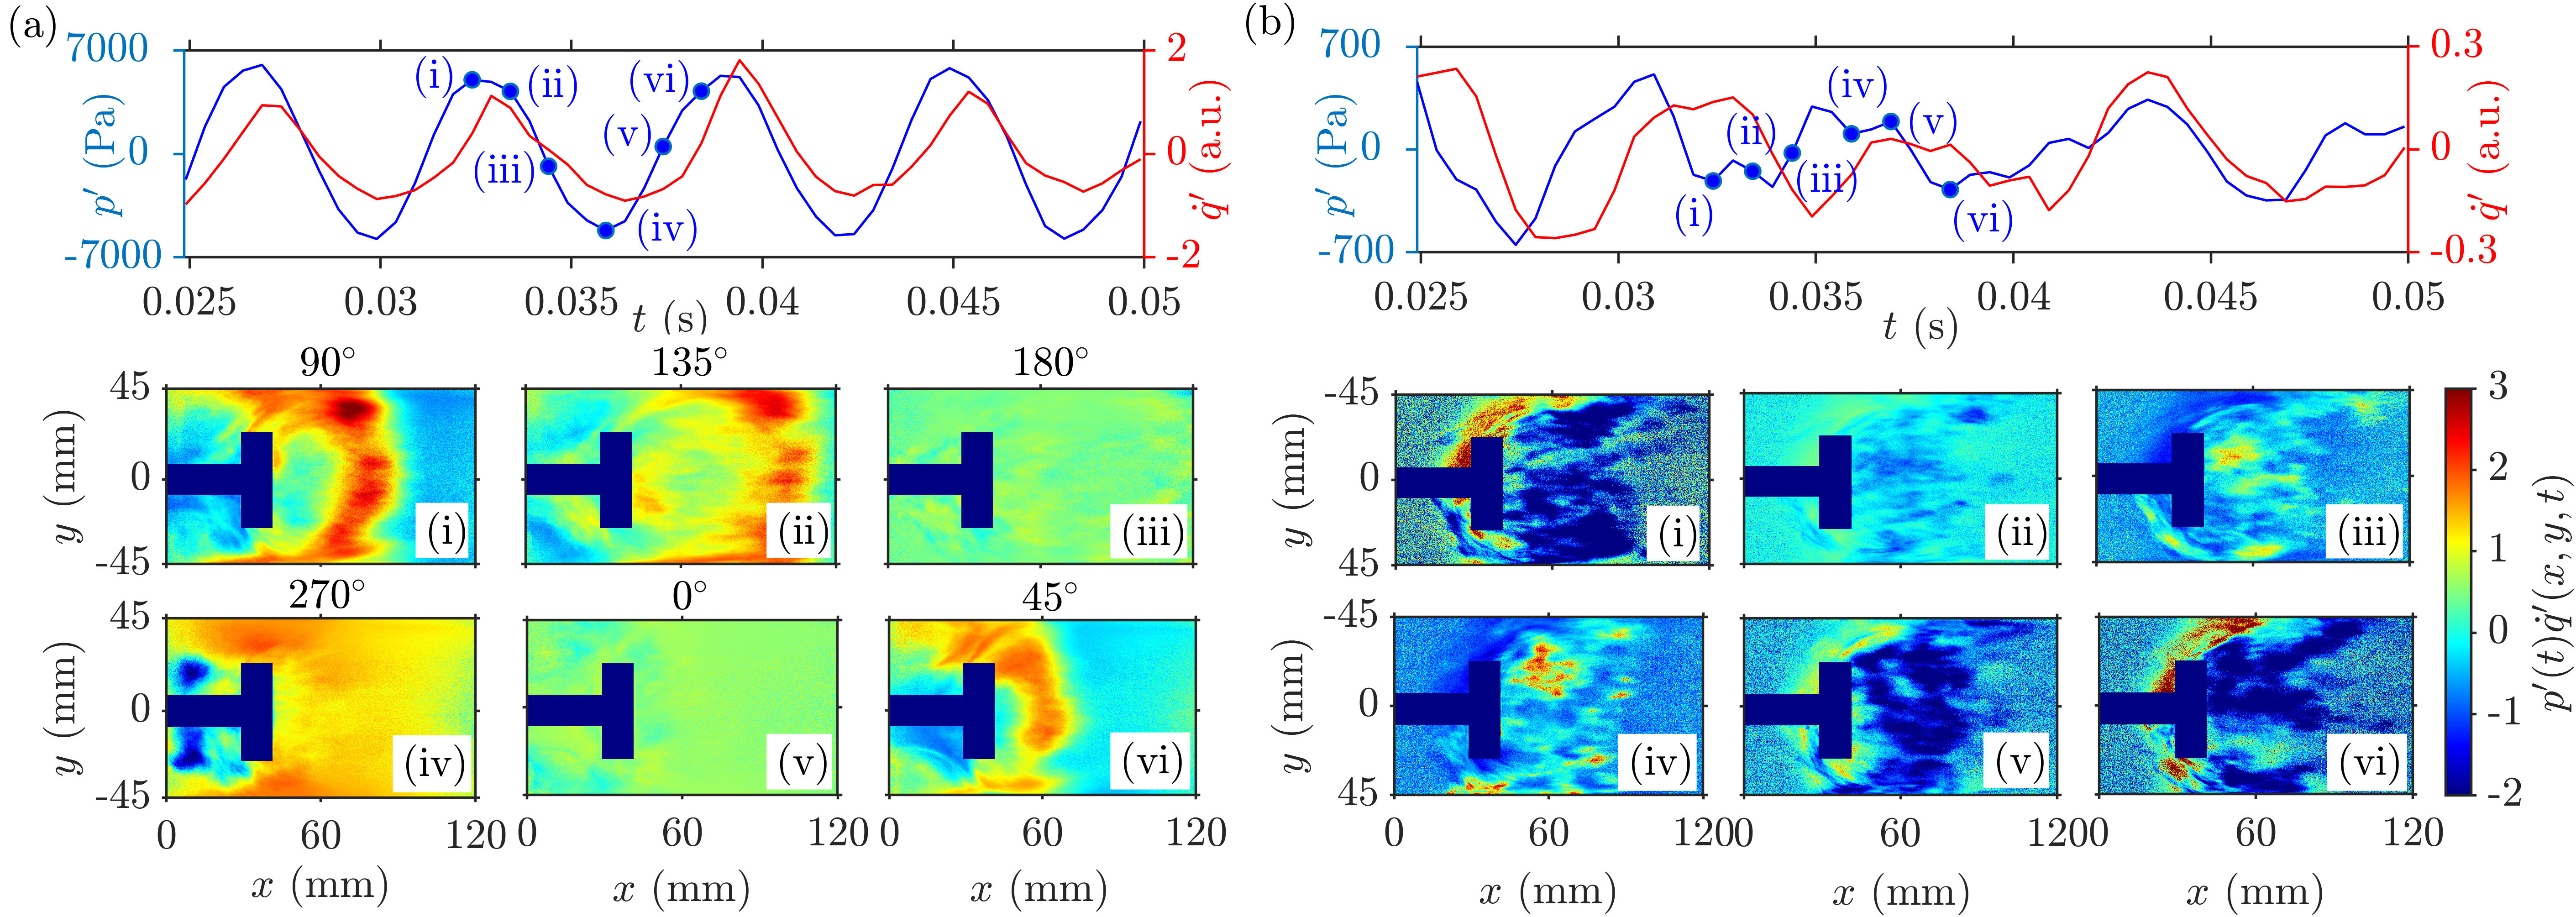
\includegraphics[width=1\textwidth]{spatio_temporal_5.png}
\caption{Time series of $p^{\prime}$ and $\dot{q}^{\prime}$ signals and (i-vi) the corresponding spatial distribution of $p^\prime(t)\dot{q}^\prime(x,y,t)$ field for  (a) phase-averaged images during the state of thermoacoustic instability and (b) instantaneous images during the state of suppression of these instabilities upon self-coupling for $L_{\text{c}} = 1600$ mm and $d_{\text{c}} = 25.4$ mm. The phase averaging in panel (a) is performed for a particular phase of $p^{\prime}$ signal, mentioned on the top of images in (a), over 20 images. }
\label{fig5}
\end{figure*}

In this section, we compare the spatiotemporal changes in the combustor as thermoacoustic instabilities are suppressed through self-coupling. During the state of thermoacoustic instability, we notice the periodic emergence of large-scale vortical structures from the dump plane of the combustor \cite{sujith2021thermoacoustic}. These vortices impinge on both the side walls of the combustor and the bluff-body. The breaking of these vortices results in the fine scale mixing of the reactants and hot products, causing a large heat release release fluctuations in the system. In contrast, during the state of complete suppression of thermoacoustic instability, we observe the absence of any such large-scale vortex in the combustor, wherein the flame dynamics appears to be nearly the same at all time instances. 

In Fig.~\ref{fig5}a(i-vi), we show the spatial distribution of $p^\prime(t) \dot{q}^\prime(x,y,t)$, i.e., local acoustic power, calculated for the phase-averaged images corresponding to the state of thermoacoustic instability. Such phase-averaged images are not shown for the state of complete suppression as the signals are aperiodic in time; as a result, we only show representative snapshots of instantaneous distribution of local acoustic power for this state in Fig. \ref{fig5}b(i-vi). The blue color in Fig. \ref{fig5}(i-vi) represents the local acoustic power sinks ($p^\prime(t) \dot{q}^\prime(x,y,t)$ $<0$), whereas the red color represents the local acoustic power sources ($p^\prime(t) \dot{q}^\prime(x,y,t)$ $>0$).

During the state of thermoacoustic instability, we observe larger coherent regions of  acoustic power sources on the top and downstream regions of the bluff-body. When both $p^\prime$ and $\dot{q}^\prime$ signals are near their local maxima (Fig. \ref{fig5}a-i,ii), these regions of acoustic power sources consist of larger magnitude and are observed as clusters in the spatial field. On the other hand, when both $p^\prime$ and $\dot{q}^\prime$ signals are near their local minima (Fig. \ref{fig5}a-iv), acoustic power sources appear to be of low magnitude and are nearly  spread over the entire combustor flow field. The local acoustic power distribution is near zero when the phase of the signal is near $180^\circ$ or $0^\circ$ (Fig. \ref{fig5}a-v,iii, respectively). Small regions of acoustic power sink are observed around the shaft of the bluff-body. Thus, the local distribution of acoustic power is highly dynamic during the state of thermoacoustic instability. 

During the state of complete suppression of thermoacoustic instability in Fig. \ref{fig5}b(i-vi), we observe that the spatial distribution of instantaneous acoustic power is highly inhomogeneous (incoherent), and its value is observed to be negative (acoustic power sinks) in the majority of the reaction field of the combustor. Therefore, we notice that the self-feedback of the acoustic field through a coupling tube of optimum length and diameter breaks the constructive interactions between the acoustic pressure and the local heat release rate oscillations in the combustor, which causes lesser thermoacoustic driving from the heat release rate field to the acoustic field of the system. As a result, the suppression of thermoacoustic instability is observed in the system.

\section{Conclusion} \addvspace{10pt}

In summary, we demonstrate the possibility of complete mitigation of thermoacoustic instability in a bluff-body stabilized turbulent combustor by inducing a delayed acoustic self-feedback in the system. This self-feedback is achieved by coupling the acoustic field of the system to itself, using a tube attached near the anti-node position of the acoustic standing wave. We observe complete suppression of thermoacoustic instability in the combustor when the length of the coupling tube is approximately 1.5 times that of the combustor (i.e., $L_{\text{c}} \approx 1.5L_{\text{duct}}$). We find that the mitigation of these instabilities is associated with a gradual decrease in the amplitude of acoustic pressure oscillations and a shift in their dominant frequency towards a lower value. Furthermore, we notice that the dynamical behavior of acoustic pressure fluctuations changes from the state of limit cycle oscillations to aperiodic oscillations via intermittent oscillations during the suppression of thermoacoustic instability. The synchronization of the acoustic pressure and global heat release rate fluctuations, observed during the uncoupled state of thermoacoustic instability, breaks down gradually and the oscillations become desynchronized as the system approaches the state of complete suppression. During this state, we do not observe any large-scale coherent structures in the reaction field of the combustor as witnessed during thermoacoustic instability. We also notice the disruption of acoustic power sources in the reaction during the state of complete suppression of oscillations, which happens due to the breaking of the local synchrony between acoustic pressure and heat release rate fluctuations in the spatial field of the combustor. 

Thus, self-coupling provides a promising control mechanism to suppress thermoacoustic instability in turbulent combustors. Unlike in traditional active closed-loop controls, we do not need to preprocess the pressure signal using any electromechanical devices in the method of self-coupling. Therefore, we believe that self-coupling opens up novel, cost-effective ways to mitigate thermoacoustic instability in practical gas turbines and rocket engines. 
 
\acknowledgement{Acknowledgments} \addvspace{10pt}
This work is supported by the J. C. Bose Fellowship (No. JCB/2018/000034/SSC) and the IoE initiative (SB/2021/0845/AE/MHRD/002696) from the Department of Science and Technology (DST), Government of India.

\bibliographystyle{pci}
\bibliography{PCI_LaTeX}

% -------------------------------------------------------------------- %
% -------------------------------------------------------------------- %
% -------------------------------------------------------------------- %

\newpage

\small
\baselineskip 10pt

% -------------------------------------------------------------------- %
% -------------------------------------------------------------------- %
% -------------------------------------------------------------------- %

% -------------------------------------------------------------------- %
% -------------------------------------------------------------------- %
% -------------------------------------------------------------------- %

\end{document}

% -------------------------------------------------------------------- %
% -------------------------------------------------------------------- %
% -------------------------------------------------------------------- %
